\documentclass[dvipdfmx,journal]{IEEEtran}

\usepackage[ruled, vlined]{algorithm2e}    % \begin{algorithm2e}
\usepackage{amsmath}        % \begin{align*}
\usepackage{amssymb}        % \mathbb{A}
\usepackage{amsthm}         % \newtheorem
\usepackage{bm,bbm}         % \bm{A}, \bbm{1}
\usepackage{booktabs}       % \toprule, \midrule, \bottomrule
\usepackage{caption}        % \captionsetup
\usepackage{enumitem}       % \begin{enumerate}[label=(\alph*)]
\usepackage{geometry}       % \geometry{margin=1in}
\usepackage{hyperref}       % \href{URL}{text}
\usepackage{ifthen}         % \ifthenelse
\usepackage{lipsum}         % \lipsum
\usepackage{mathrsfs}       % \mathscr{A}
\usepackage{mathtools}      % \mathrlap
\usepackage{optidef}        % \begin{mini*}{x}{f(x)}{}{}
\usepackage{orcidlink}      % \orcidlink
\usepackage{physics}        % \qty, \norm, \abs
\usepackage{subfiles}       % \subfile{file}
\usepackage{thm-restate}    % \begin{restatable}{theorem}{thm}
\usepackage{tikz}           % \begin{tikzpicture}
\usepackage{xparse}         % \NewDocumentCommand
% \usepackage{calc}         % \setlength
% \usepackage{cancel}       % \cancel
% \usepackage{parskip}      % \setlength{\parskip}{0.5em}
% \usepackage{csvsimple}    % \csvautotabular
% \usepackage{diagbox}      % \diagbox
% \usepackage{dsfont}       % \mathds{1}
% \usepackage{epsfig}       % \epsfig
% \usepackage{fancybx}      % \ovalbox
% \usepackage{float}        % \begin{figure}[H]
% \usepackage{lipsum}       % \lipsum
% \usepackage{listings}     % \begin{lstlisting}
% \usepackage{makecell}     % \makecell{L1\L2}
% \usepackage{multicol}     % \begin{multicols}{2}
% \usepackage{multirow}     % \multirow
% \usepackage{nicematrix}   % \begin{NiceMatrix}
% \usepackage{qcircuit}     % \Qcircuit
% \usepackage{siunitx}      % \SI{1}{\second}
% \usepackage{stfloats}     % \begin{figure*}
% \usepackage{subcaption}   % \begin{subfigure}
% \usepackage{ulem}         % \sout
% \usepackage[hyphens]{url} % \url
% \usepackage{wrapfig}      % \begin{wrapfigure}
% \usepackage[all]{xy}      % \xymatrix
% \usepackage[dvipdfmx]{graphicx}
% \usepackage[square, sort, comma, numbers]{natbib}

\geometry{margin=1in}
\hypersetup{colorlinks=true,linkcolor=blue,citecolor=blue,urlcolor=blue}

\definecolor{cA}{HTML}{0072BD}
\definecolor{cB}{HTML}{EDB120}
\definecolor{cC}{HTML}{77AC30}
\definecolor{cD}{HTML}{D95319}

\newcommand{\red}[1]{\textcolor{red}{#1}}
\newcommand{\blue}[1]{\textcolor{blue}{#1}}
\newcommand{\cyan}[1]{\textcolor{cyan}{#1}}
\newcommand{\gray}[1]{\textcolor{gray}{#1}}
\newcommand{\green}[1]{\textcolor{green}{#1}}
\newcommand{\brown}[1]{\textcolor{brown}{#1}}
\newcommand{\black}[1]{\textcolor{black}{#1}}
\newcommand{\st}{\text{ s.t. }}
\newcommand{\Img}[1]{\mathrm{Im}\qty(#1)}
\newcommand{\Ker}[1]{\mathrm{Ker}\qty(#1)}
\newcommand{\Supp}[1]{\mathrm{supp}\qty(#1)}
\newcommand{\Rank}[1]{\mathrm{rank}\qty(#1)}
\newcommand{\floor}[1]{\left\lfloor #1 \right\rfloor}
\newcommand{\ceil}[1]{\left\lceil #1 \right\rceil}
% C++ (https://tex.stackexchange.com/questions/4302/prettiest-way-to-typeset-c-cplusplus)
\newcommand{\Cpp}{C\nolinebreak[4]\hspace{-.05em}\raisebox{.4ex}{\relsize{-3}{\textbf{++}}}}
% https://tex.stackexchange.com/questions/28836/typesetting-the-define-equals-symbol
\newcommand{\defeq}{\coloneqq}
\newcommand{\eqdef}{\eqqcolon}
% https://tex.stackexchange.com/questions/5502/how-to-get-a-mid-binary-relation-that-grows
\newcommand{\relmiddle}[1]{\mathrel{}\middle#1\mathrel{}}
\newcommand{\Lhopital}{L'H\^optial}

\DeclareMathOperator{\Proj}{Proj}
\DeclareMathOperator{\Exp}{Exp}
\DeclareMathOperator{\Hess}{Hess}
\DeclareMathOperator{\Retr}{Retr}
\DeclareMathOperator{\Span}{span}
% \DeclareMathOperator{\myGrad}{grad}
% \renewcommand{\grad}{\myGrad}

% https://tex.stackexchange.com/questions/564216/newcommand-for-each-letter
\ExplSyntaxOn
\NewDocumentCommand{\definealphabet}{mmmm}{
\int_step_inline:nnn{`#3}{`#4}{
\cs_new_protected:cpx{#1 \char_generate:nn{##1}{11}}{
\exp_not:N #2{\char_generate:nn{##1}{11}}}}}
\ExplSyntaxOff

\definealphabet{bb}{\mathbb}{A}{Z}
\definealphabet{rm}{\mathrm}{A}{Z}
\definealphabet{cal}{\mathcal}{A}{Z}
\definealphabet{frak}{\mathfrak}{a}{z}
% \definealphabet{scr}{\mathscr}{A}{Z}
% \definealphabet{frak}{\mathfrak}{A}{Z}

\newtheorem{theorem}{Theorem}
\newtheorem{proposition}{Proposition}
\newtheorem{lemma}{Lemma}
\newtheorem{definition}{Definition}
\newtheorem{corollary}{Corollary}
\newtheorem{remark}{Remark}
\newtheorem{example}{Example}
\newtheorem{assumption}{Assumption}

% https://qiita.com/rityo_masu/items/efd44bc8f9229e014237
\allowdisplaybreaks[4]

% \lstset{
%   language=Python,numbers=left,frame=single,breaklines=true,lineskip=-0.9ex,xleftmargin=3zw,xrightmargin=0zw,
%   basicstyle=\ttfamily,ndkeywordstyle=\small,identifierstyle=\small,numberstyle=\scriptsize,
%   commentstyle=\color[rgb]{0,0.6,0},stringstyle=\small\ttfamily\color[rgb]{0.89,0.55,0},keywordstyle=\small\bfseries\color[rgb]{0.28,0.28,0.95},
% }

\usetikzlibrary{
  3d,
  % fit,
  calc,
  math,
  matrix,
  patterns,
  backgrounds,
  arrows.meta,
  shapes.geometric,
  % decorations.pathmorphing,
}

% \graphicspath{{./fig/}}

% \providecommand{\main}{.}
\newboolean{isMain}
\setboolean{isMain}{true}

\begin{document}

\title{Fruchterman--Reingold Algorithm with Random Subspace Newton}
\author{Hiroki Hamaguchi\,\orcidlink{0009-0005-7348-1356}}
\date{\today}
\maketitle

\begin{abstract}
  The abstract goes here.
  \lipsum[1]
\end{abstract}

\begin{IEEEkeywords}
  Graph drawing, Fruchterman--Reingold algorithm, Random Subspace method.
\end{IEEEkeywords}

\section{Introduction}

\IEEEPARstart{G}{raph} is a mathematical structure representing pairwise relationships between objects, and graph drawing is one of the most fundamental tasks in data science. Indeed, Numerous general algorithms have been proposed for graph drawing~\cite{tutteHowDrawGraph1963,chrobakLineartimeAlgorithmDrawing1995,sugiyamaMethodsVisualUnderstanding1981,ghassemitoosiSimulatedAnnealingPreProcessing2016}
Among these, one of the most popular strategies is force-directed algorithms.

In force-directed algorithms, the graph is modeled as a physical system of particles. These include methods such as the Kamada--Kawai (KK) layout~\cite{kamadaAlgorithmDrawingGeneral1989} using shortest path distances for a cost function, and the Fruchterman--Reingold (FR) layout~\cite{fruchtermanGraphDrawingForcedirected1991}, which is the primary focus of this paper.

The FR algorithm is one of the most widely used force-directed algorithms. It is also implemented in many modern graph drawing libraries such as NetworkX~\cite{osti_960616}, Graphviz~\cite{ellsonGraphvizOpenSource2002}, and igraph~\cite{csardiIgraphSoftwarePackage2006}. The FR layout is based on a physical model of a system of particles and springs, and FR algorithm seeks the equilibrium of the forces between nodes.

However, since both the KK layout and the FR layout requires to compute the forces or energies between all pairs of vertices, they have a high computational cost of $\order{n^2}$ per iteration, where $n$ is the number of vertices in the graph. To address this kind of computational burden, several methods have been proposed. One strategy is to approximate the $n$-body simulation using hierarchical methods such as the fast multipole method~\cite{greengardFastAlgorithmParticle1987}, the Barnes--Hut approximation~\cite{barnesHierarchicalLogForcecalculation1986}, multilevel approaches~\cite{Hu2006EfficientHF}, or stress majorization~\cite{gansnerGraphDrawingStress2005}.

Another approach is to accelerate the optimization algorithm directly, which aligns with the spirit of our work. Recent researches have accelerated the algorithms for FR layout and KK layout through various methods, including GPU parallel architectures~\cite{gajdosParallelFruchtermanReingold2016}, numerical optimization techniques such as L-BFGS~\cite{6183577}, and Stochastic Gradient Descent (SGD)~\cite{8419285}.

Based on such advances, in this paper, we investigate the ability of another algorithm: Random Subspace Newton (RSN). The RSN method is a variant of the Newton method that uses a random subspace to approximate the Hessian matrix. The RSN method and its variant have been proposed in the context of optimization problems~\cite{NEURIPS2019_bc6dc48b,fujiRandomizedSubspaceRegularized2022,cartisRandomisedSubspaceMethods2022,higuchiFastConvergenceSecondOrder2024}.

\begin{table}[t]
  \centering
  \begin{tabular}{cc}
    \large{\textbf{FR}}                                                                                                                & \large{\textbf{L-BFGS}}   \\
    \begin{minipage}{0.45\columnwidth}
      \centering
      \includegraphics[width=\columnwidth]{/home/hari64boli64/University/FruchtermanReingoldByRandomSubspace/doc/jagmesh1_FR_50iter.png}
    \end{minipage} &
    \begin{minipage}{0.45\columnwidth}
      \centering
      \includegraphics[width=\columnwidth]{/home/hari64boli64/University/FruchtermanReingoldByRandomSubspace/doc/jagmesh1_LBFGS_50iter.png}
    \end{minipage}                           \\
    \large{\textbf{proposed}}                                                                                                          & \large{\textbf{+ L-BFGS}} \\
    \begin{minipage}{0.45\columnwidth}
      \centering
      \includegraphics[width=\columnwidth]{/home/hari64boli64/University/FruchtermanReingoldByRandomSubspace/doc/jagmesh1_LBFGS_50iter.png}
    \end{minipage}
                                                                                                                                       &
    \begin{minipage}{0.45\columnwidth}
      \centering
      \includegraphics[width=\columnwidth]{/home/hari64boli64/University/FruchtermanReingoldByRandomSubspace/doc/jagmesh1_LBFGS_50iter.png}
    \end{minipage}
  \end{tabular}
  \begin{tikzpicture}[overlay, remember picture]
    \draw[->, thick] (-0.3,1.3) -- (+0.3,1.3);
  \end{tikzpicture}
  \caption{Comparison of the FR algorithm (left, NetworkX) and L-BFGS-B (right, my implementation) on the \texttt{jagmesh1} dataset.}
  \label{table:four_images}
\end{table}

The rest of the paper is organized as follows.
In Section~\ref{sec:preliminary}, we define the optimization problem for the FR algorithm.
In Section~\ref{sec:RSN}, we introduce the Random Subspace method and report a its problem when directly applied to the FR algorithm.
In Section~\ref{sec:algorithm}, we propose a new algorithm that combines the FR algorithm with the Random Subspace method.
In Section~\ref{sec:experiment}, we present the experimental results.
Finally, we conclude and discuss future work in Section~\ref{sec:discussion}.

\section{Preliminary}\label{sec:preliminary}

\begin{figure*}[t]
  \begin{minipage}{0.49\hsize}
    \centering
    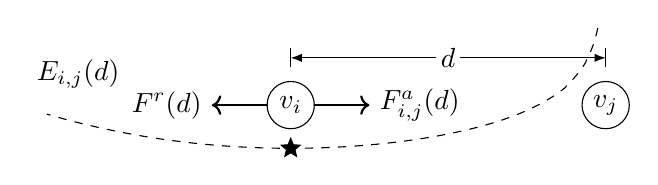
\begin{tikzpicture}
      \def\d{4}
      \def\r{0.3}
      \def\u{1.0}
      \coordinate (M1) at (0,0);
      \coordinate (M2) at (\d,0);

      \draw (M1) circle(\r) node {$v_i$};
      \draw (M2) circle(\r) node {$v_j$};

      \draw (0,+1.6*\r) -- (0,+2.4*\r);
      \draw (\d,+1.6*\r) -- (\d,+2.4*\r);
      \draw[{Latex[length=4,width=3]}-{Latex[length=4,width=3]}] ($(M1)+(90:2*\r)$) -- ($(M2)+(90:2*\r)$)
      node[midway,circle,fill=white,inner sep=0] {$d$};

      \draw[->,thick,line cap=round] (+\r,0) -- (+\u,0) node[right] {$F_{i,j}^a(d)$};
      \draw[->,thick,line cap=round] (-\r,0) -- (-\u,0) node[left] {$F^r(d)$};

      \draw[dashed,domain=3.9:-3.1,samples=1000,smooth,variable=\x] plot(\x,{-0.7+(pow((\d-\x)/\d,3)/3-ln((\d-\x)/\d))/2.2});
      \node [star,
        minimum size=0.25cm,
        star point ratio=2.25,
        inner sep=0pt,
        draw, fill=black]
      at (0,{-0.7+(1/3)/2.2}) {};

      \node at (-2.7,0.4) {$E_{i,j}(d)$};
    \end{tikzpicture}
    \caption{
      Fruchterman--Reingold model.
      The equilibrium of the attractive force $F_{i,j}^a(d)$ and the repulsive force $F^r(d)$ is the optimal distance $d=k/\sqrt[3]{w_{i,j}}$.
    }
  \end{minipage}
  \begin{minipage}{0.49\hsize}
    \centering
    \includegraphics[width=\columnwidth]{energy_3d.png}
    \caption{Energy function $E_{i,j}(d)$ for $w_{i,j} = 1$ and $k = 1$. Although $E_{i,j}$ is convex for $d$, but not for $x_i$ and $x_j$.}
    \label{fig:label}
  \end{minipage}
\end{figure*}

Firstly, in this section, we formulate the FR layout as a continuous optimization problem, and introduce the conventional approaches to this problem, namely the FR algorithm and the L-BFGS algorithm.

\subsection{Fruchterman--Reingold layout}

Let us define
$\bbR_{> 0} \defeq \qty{ x \in \bbR \mid x > 0 }, \quad \bbR_{\geq 0} \defeq \qty{ x \in \bbR \mid x \geq 0 }$,
and let $W = (w_{i,j}) \in \bbR_{\geq 0}^{n \times n}$ be an adjacency matrix of a undirected connected graph $G = (V, E)$. $V = \qty{v_i \mid 1 \leq i \leq n}$ is a set of vertices and $E = \qty{(v_i, v_j) \mid w_{i,j} > 0}$ is a set of edges. We call $w_{i,j}$ as a weight of the edge $(v_i, v_j)$.

The FR algorithm in NetworkX, for example, can handle directed unconnected graphs with $w_{i,j} < 0$, but we will not consider such cases here.
For directed graphs, slight modifications of algorithms or converting them to undirected graphs may be effective. For unconnected graphs, algorithms can be applied to each connected component independently. When some weights $w_{i,j}$ are negative, the optimization problem may become unbounded, but with $w_{i,j} >0$, the problem is always bounded and solvable.

Each vertex $v_i \in V$ is assigned to a point on a plane $x_i \in \bbR^2$ and we define $x = (x_1, \dots, x_n) \in \bbR^{2 \times n}$ as the configuration of the graph.
For an parameter $k$ and a distance $d_{i,j} \defeq \norm{x_i - x_j}_2$ between two vertices $v_i$ and $v_j$, Fruchterman and Reingold~\cite{fruchtermanGraphDrawingForcedirected1991} defined the power of attraction $F_{i,j}^a: \bbR_{> 0} \to \bbR$ and the power of repulsion $F^r: \bbR_{> 0} \to \bbR$ as
\begin{equation*}
  F_{i,j}^a(d) \defeq \frac{w_{i,j} d^2}{k}, \quad F^r(d) \defeq -\frac{k^2}{d}.
\end{equation*}
We refer this Force-Directed layout as the Fruchterman--Reingold (FR) layout.
The energy for these powers $E_{i,j}(d)$ can be defined as
\begin{align*}
  E_{i,j}(d) & \defeq \int_{0}^{d} F_{i,j}^a(r) \dd{r} + \int_{\infty}^{d} F^r(r) \dd{r} \\
             & = \frac{w_{i,j} d^3}{3k} - k^2\log{d}.
\end{align*}
As a remark, the energy function $E_{i,j}$ is convex for $d$ and minimized when $d^* = k/\sqrt[3]{w_{i,j}}$, but it is not Lipschitz continuous, and is not convex for $x_i$ (?correct expression?). Refer to Figure~\ref{fig:label}.

Now, the optimization problem for FR layout can be formulated as the minimization of the energy function $f: \bbR^{2 \times n} \to \bbR$, as known as a stress of the graph:
\begin{mini}
  {x \in \bbR^{2 \times n}}
  {f(x) \defeq \sum_{i<j} E_{i,j}(d_{i,j})}
  {\label{eq:fr}}
  {}
\end{mini}

\subsection{Fruchterman--Reingold algorithm}

The most standard approach to solve the optimization problem~\eqref{eq:fr} is the Fruchterman--Reingold algorithm~\cite{fruchtermanGraphDrawingForcedirected1991}, the original force-directed algorithm for graph drawing. Let us consider this algorithm in the context of the optimization problem~\eqref{eq:fr}.
As pointed out in~\cite{tunkelang1999numerical},
the FR algorithm can be regarded as a gradient descent method for the energy function $f$ with cooling schedule.

Let denote $f_i(x): \bbR^2 \to \bbR$ as the energy function for the vertex $v_i$:
\begin{equation*}
  f_i(x_i) \defeq \sum_{j \neq i} E_{i,j}(d_{i,j}).
\end{equation*}
The gradient and Hessian (for later sections) of $f_i$ are
\begin{gather*}
  \nabla f_i(x_i) = \sum_{j \neq i} \qty(\frac{w_{i,j}d_{i,j}}{k} - \frac{k^2}{d_{i,j}^2}) (x_i-x_j), \\
  \nabla^2 f_i(x_i) = \sum_{j \neq i} \qty(\frac{w_{i,j}d_{i,j}}{k} - \frac{k^2}{d_{i,j}^2}) I_d +      \\
  \sum_{j \neq i} \qty(\frac{w_{i,j}}{k d_{i,j}} + \frac{2k^2}{d_{i,j}^4}) (x_i - x_j)(x_i - x_j)^\top.
\end{gather*}

The pseudo code of the FR algorithm is as follows:
\begin{algorithm}[ht]
  \caption{Fruchterman--Reingold algorithm}
  \label{alg:fr}
  \KwIn{Graph $G = (V, E)$ with its weights $W$}
  \KwOut{Point configuration $x \in \bbR^{2 \times n}$}

  $\text{define parameters } k, t, dt, \text{iterations}$\;
  $x_i \gets \text{random}$ for all $v_i \in V$\;
  \For{$j \gets 0$ \KwTo \textit{iterations}}{
    $\text{compute gradient } \nabla f_i(x_i)$ for all $v_i \in V$\;
    $x_i \gets x_i + t \frac{\nabla f_i(x_i)}{
        \norm{\nabla f_i(x_i)}_{2}}$ for all $v_i \in V$\;
    $t \gets t - dt$\;
    \If{\text{convergence condition}}{
      \textbf{break}\;
    }
  }
  \Return $\text{pos}$
\end{algorithm}

Algorithm~\ref{alg:fr} is based on the original implementation~\cite{fruchtermanGraphDrawingForcedirected1991} and implementation in NetworkX~\cite{osti_960616}.
The $t$ in the parameter represents the temperature, which is used to control the step size of the gradient descent. This temperature assures the convergence to a certain configuration, which might not be a local minimum of the energy function. There are some ways to define the parameters or cooling schedule, such as linear cooling, exponential cooling, or adaptive cooling.

\subsection{L-BFGS algorithm}

Another approach to solve the optimization problem~\eqref{eq:fr} is to use the L-BFGS algorithm~\cite{6183577}, which is a quasi-Newton method that approximates the Hessian matrix using the gradient information. The L-BFGS algorithm is widely used in optimization problems, and there are many implementations available, such as SciPy~\cite{2020SciPy-NMeth} and C++ L-BFGS~\cite{liuLimitedMemoryBFGSMethod2019}.

For the optimization problem~\eqref{eq:fr}, the L-BFGS algorithm can be applied via flattening the configuration $x$ to a vector $x \in \bbR^{2n}$.

\section{Random Subspace Newton}\label{sec:RSN}

In this section, we introduce the Random Subspace Newton (RSN) method and report a its problem when directly applied to the FR algorithm.

\subsection{What is Random Subspace Newton}

First, we introduce the RSN method.
RSN is a variant of the Newton's method.
For $N$ variables problem, the Newton's method requires to compute the Hessian matrix of size $N \times N$ at each iteration, which poses a high computational cost for large-scale problems.
One way to address this issue is to employ quasi-Newton methods, such as the L-BFGS method, which approximates the Hessian directly, and has also been applied in graph drawing~\cite{6183577}.
In contrast, RSN focuses on a subspace of dimension $S$ randomly selected from the solution space and utilizes the exact Hessian matrix of size $S \times S$ defined on this subspace.
Since $S \ll N$, the computational cost per iteration is significantly reduced.

The RSN method resembles the stochastic coordinate descent method, which updates only a subset of the variables at each iteration using gradient information. The difference is that RSN uses the Hessian matrix to determine the update direction, bringing the method closer to the Newton method.

Moreover, recent studies have explored its application not only to convex optimization problems but also to non-convex optimization problems~\cite{fujiRandomizedSubspaceRegularized2022}.

\subsection{Random Subspace Newton for FR Algorithm}

In this way, the problem exhibits a natural affinity with the RSN method, as it inherently defines a subspace of the solution space for the FR layout.

Moreover, the effectiveness of Stochastic Gradient Descent (SGD) for KK layout is well-documented in~\cite{8419285}.
In contrast to the KK layout, where each function is individually determined by $\frac{k_{i,j}}{2}(d_{i,j}-l_{i,j})^2$ based on the actual distance between vertices $d_{i,j}$ and their optimal distance $l_{i,j}$, the FR layout assigns the same value, $-k^2\log{d_{i,j}}$, to all pairs of points without direct edges, making SGD relatively less effective for the FR layout.

However, the report in the KK layout, which highlights that optimization focusing on each edge yields favorable results, suggests that optimization focusing on each vertex, such as methods utilizing RSN, may also be effective in the FR layout.

In this situation, our research aims to investigate the effectiveness of the RSN method for the FR layout.

\subsection{problem of RSN for FR Algorithm}

\begin{figure*}[t]
  \centering
  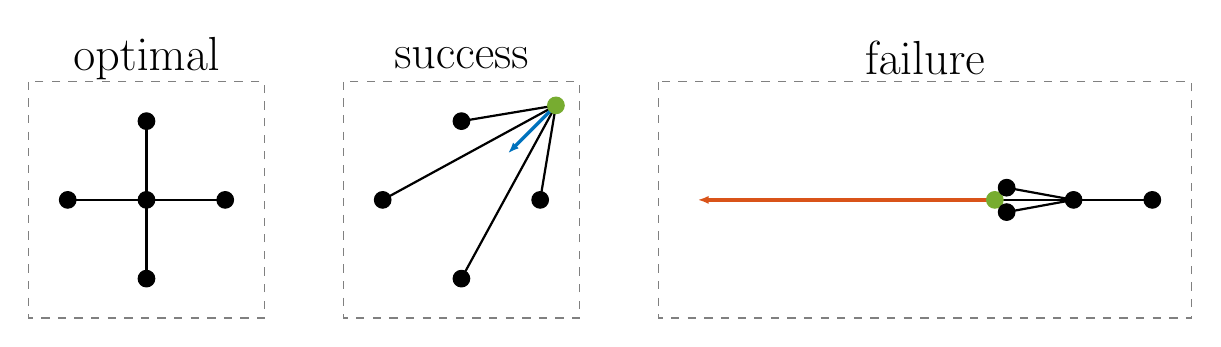
\begin{tikzpicture}
    \foreach \xA/\yA/\xB/\yB/\xC/\yC/\xD/\yD/\xE/\yE/\arrowX/\arrowY/\xShift/\xRect/\arrowV/\caZero/\caOne/\desc in {
        0/0/-1/0/0/1/0/-1/1/0/0/0/0/-1.5/a0/black/black/optimal,
        1.2/1.2/-1/0/0/1/0/-1/1/0/0.592271758813887/0.592271758813887/4/-1.5/a0/cC/black/success,
        0/0/-1/0/-0.85/0.155/-0.85/-0.155/1/0/-4.77422/0/11.77422/-5.27422/a1/black/cC/failure}{
        \begin{scope}[xshift=\xShift cm]
          \draw[dashed,color=gray,line width=0.5pt] (\xRect, 1.5) rectangle (1.5, -1.5);
          \node at ({(\xRect+1.5)/2}, 1.8) {\LARGE{\desc}};
          \coordinate (a0) at (\xA, \yA);
          \coordinate (a1) at (\xB, \yB);
          \coordinate (a2) at (\xC, \yC);
          \coordinate (a3) at (\xD, \yD);
          \coordinate (a4) at (\xE, \yE);
          \draw[thick] (a0) -- (a1);
          \draw[thick] (a0) -- (a2);
          \draw[thick] (a0) -- (a3);
          \draw[thick] (a0) -- (a4);

          \ifthenelse{\equal{\arrowX}{0} \AND \equal{\arrowY}{0}}{}{
          \ifthenelse{\equal{\desc}{success}}{
          \draw[-{Latex[length=4,width=3]},very thick,cA] (\arrowV) -- (\arrowX, \arrowY);
          }{
          \draw[-{Latex[length=4,width=3]},very thick,cD] (\arrowV) -- (\arrowX, \arrowY);
          }}

          \filldraw[draw=\caZero,fill=\caZero] (a0) circle (3pt);
          \filldraw[draw=\caOne,fill=\caOne]   (a1) circle (3pt);
          \filldraw[draw=black,fill=black] (a2) circle (3pt);
          \filldraw[draw=black,fill=black] (a3) circle (3pt);
          \filldraw[draw=black,fill=black] (a4) circle (3pt);
        \end{scope}
      }
  \end{tikzpicture}
  \caption{
    Visualization of the problem of the subspace method.
    Let a graph as shown in the left (optimal), where $k$ and all positive edge weights $w_{i,j}$ are set to 1.
    For the situation in the middle (success), the RSN works effectively.
    However, in the situation depicted on the right (failure),
    where the points are set as $x_0=(0,0), x_1=(-1,0), x_2=(-0.85,0.155), x_3=(-0.85,-0.155), x_4=(1,0)$,
    the Hessian for the subspace of $x_1$ is approximately
    $
      \begin{pmatrix} 1.841 & 0 \\ 0 & 1.159 \end{pmatrix}
    $.
    This Hessian, while positive definite and not ill-conditioned, leads to a Newton direction that clearly deviates significantly from the global optimal solution.
  }
  \label{fig:why_RSN_failed}
\end{figure*}

However, unfortunately, the RSN method is not necessarily effective for the FR layout.
As shown in Figure \ref{fig:why_RSN_failed}, although the energy function \( f_i \) with respect to the position \( x_i \) of each vertex is convex in the FR layout, the overall energy function \( f \) with respect to \( x_i \) is not convex.

\section{Algorithm} \label{sec:algorithm}


\section{Experiment} \label{sec:experiment}

We used dataset from \cite{davis2011university} and MatrixMarket \cite{boisvertMatrixMarketWeb1997}.

\url{https://reference.wolfram.com/language/tutorial/GraphDrawingIntroduction.html}

\section{Discussion} \label{sec:discussion}

In this paper, we investigated the effectiveness of the Random Subspace Newton method for the Fruchterman--Reingold algorithm.

\subsection{Combination with Other Methods}



\subsection{Application to Other Problems}



\section{Acknowledgment}

The author would like to express our sincere gratitude to PL Poirion and Andi Han for their insightful discussions, which have greatly inspired and influenced this research.

\ifthenelse{\boolean{isMain}}{
  \bibliographystyle{IEEEtran}
  \bibliography{FruchtermanReingoldByRandomSubspace}
}{}

\appendices

\section{Optimal Scaling}

When we optimize a placement for FR-layout with an initial placement obtained, for instance through KK-layout, scaling the initial placement at first can often yield better results than directly using the unmodified initial placement.
In this section, we address the problem of finding the optimal scaling factor that minimizes the energy function for a given configuration.

\subsection{Optimal Scaling Algorithm}

Formulating the optimization through scaling, the task reduces to selecting an appropriate scaling factor $x \in \bbR_{> 0}$ that minimizes the following energy function:

\begin{align*}
  \phi(x) \defeq {} & \qty(\sum_{i < j} \frac{w_{ij} (xd_{ij})^3}{3k}) - k^2 \sum_{i < j} \log(x d_{ij})                                    \\
  \begin{split}
    = {} & x^3 \qty(\sum_{i < j} \frac{w_{ij} d_{ij}^3}{3k}) - \log(x)(k^2 n(n-1))\\
    & - k^2 \sum_{i < j} \log(d_{ij})
  \end{split} \\
  \phi'(x) = {}     & 3x^2 \qty(\sum_{i < j} \frac{w_{ij} d_{ij}^3}{3k}) - \frac{k^2 n(n-1)}{x}                                             \\
  \phi''(x) = {}    & 6x \qty(\sum_{i < j} \frac{w_{ij} d_{ij}^3}{3k}) + \frac{k^2 n(n-1)}{x^2}
\end{align*}

The function $\phi(x)$ is convex, and we can find the optimal scaling factor $x$ by using Newton's method.

This algorithm achieves sufficient convergence within a few iterations, and when we pre-compute the coefficients of $\phi(x)$ with $w_{i,j} > 0$, the time complexity is just $\order{\abs{E}}$.

\section{Another approach based on the Hexagonal Lattice}

todo

\end{document}